%
%
% Used for displaying a sample figure. If possible, figure files should
% be included in EPS format.
%
% If you use the hyperref package, please uncomment the following line
% to display URLs in blue roman font according to Springer's eBook style:
% \renewcommand\UrlFont{\color{blue}\rmfamily}
%!TeX root = paper22-ieee-internet-si-decentralised-systems.tex

\lstdefinelanguage{scala}{
  keywords={abstract,case,catch,class,def,%
    do,else,extends,false,final,finally,%
    for,if,implicit,import,match,mixin,%
    new,null,object,override,package,%
    private,protected,requires,return,sealed,%
    super,this,throw,trait,true,try,lazy,%
    type,val,var,while,with,yield,forSome},
  otherkeywords={=>,<-,<\%,<:,>:,\#},
  sensitive=true,
  columns=fullflexible,
  morecomment=[l]{//},
  morecomment=[n]{/*}{*/},
  morestring=[b]",
  stringstyle=\ttfamily\color{red!50!brown},
  showstringspaces=false,
  morestring=[b]',
  morestring=[b]""",
  basicstyle=\sffamily\lst@ifdisplaystyle\scriptsize\fi\ttfamily,
  emphstyle=\sffamily\bfseries\ttfamily
}
\definecolor{ddarkgreen}{rgb}{0,0.5,0}
\lstdefinelanguage{scafi}{
  frame=single,
  basewidth=0.5em,
  language={scala},
  keywordstyle=\color{blue}\textbf,
  commentstyle=\color{ddarkgreen},
  keywordstyle=[2]\color{red}\textbf,
  keywords=[2]{rep,nbr,foldhood,foldhoodPlus,aggregate,branch,spawn,mux,mid},
  keywordstyle=[3]\color{gray},
  keywords=[3]{Me,AroundMe,Everywhere,Forever}, %,@@,@@@
  keywordstyle=[4]\color{red}\textbf,
  keywords=[4]{in,out,rd},
  keywordstyle=[5]\color{violet},
  keywords=[5]{evolve,when,andNext,workflow,G,C,broadcast,gossip},
  keywordstyle=[6]\color{orange},
  keywords=[6]{Available,Serving,Done,Waiting,Removing,None,Set}
}

\lstset{language=scafi}
% Please use the

\newcommand{\MacroSwarm}{{\sc{}MacroSwarm}}


%% Page limit: 7-15 pages (without counting references)
\newcommand{\meta}[1]{{\color{blue} #1}}%
%\chapter{\MacroSwarm{} Swarm Programming Framework}
\chapter{\MacroSwarm{}}

%
\section{Introduction}

Recent technological advances 
 foster a vision of \emph{swarms} of mobile cyber-physical agents able to compute, coordinate with neighbours, and interact with the environment according to increasingly complex patterns, plans, and goals.
%
Notable examples include swarms of drones and robots~\cite{DBLP:journals/firai/SchranzUSE20}, 
 fleets of vehicles~\cite{DBLP:journals/jiii/TahirBHTP19},
 and crowds of wearable-augmented people~\cite{DBLP:journals/wc/GalininaMH0K18}.
%
In these domains,
 a prominent research problem
 is how to effectively engineer \emph{swarm behaviour}~\cite{DBLP:journals/swarm/BrambillaFBD13},
 i.e., how to promote 
 the emergence of desired global-level outcomes %(or the accomplishment of joint goals) 
 with inherent robustness and resiliency to changes and faults in the swarm or the environment.
%
Complex patterns can emerge through the interaction of simple agents~\cite{bonabeau1999swarmintelligence-book}, and centralized approaches %of decision-making 
 can suffer from scalability and dependability issues: as such,  
 we seek for an approach based on %adopting 
 suitable distributed coordination models and languages to steer the micro-level activity of a possibly large set of agents.
%
This %general approach 
 direction has been explored by various research threads related to coordination
 like  \emph{macroprogramming}~\cite{Casadei2023,regiment}, 
 \emph{spatial computing}~\cite{SpatialIGI2013},
 \emph{ensemble languages}%\emph{attribute-based communication}
~\cite{scel2014taas,abd2020programming-cas-attribute-based}, 
 \emph{field-based coordination}~\cite{DBLP:journals/corr/Lluch-LafuenteL16,Mamei:2004a}, and \emph{aggregate computing}~\cite{DBLP:journals/jlap/ViroliBDACP19}. 
 
%
Though a number of approaches and languages have been proposed 
 for specifying or programming swarm behaviour~\cite{Meld2007,%
DBLP:conf/icra/CarrollNS21,%
paros,%
DBLP:conf/isola/KosakHBWHR20,%
Koutsoubelias2016tecola,%
lima2018dolphin,%
Mottola2014voltron,%
DBLP:conf/iros/PinciroliB16,%
DBLP:conf/iros/YiDLD0WY20},
 a key feature that is generally missing or provided only to a limited extent
 is \emph{compositionality},
 namely the ability of combining blocks of simple swarm behaviour to construct swarm systems of increasing complexity in a controlled/engineered way.
%
Additionally, most of existing approaches tend to be pragmatic, not formally-founded and quite ad-hoc: they 
 enable construction of certain types of swarm applications
 but with limited support for analysis and principled design of complex applications (e.g.~\cite{lima2018dolphin,paros,DBLP:conf/iros/PinciroliB16,DBLP:conf/icra/CarrollNS21}).
%
Exceptions that provide a formal approach exist, but they are typically overly abstract, requiring additional effort to actually code and execute swarm control programs~\cite{DBLP:journals/csur/LuckcuckFDDF19}.

The goal of this work is 
 to introduce a formally-grounded \ac{api},
 expressive and practical enough
 to concisely and elegantly encode a wide array of swarm behaviours.
%
This is based on the field-based coordination paradigm~\cite{DBLP:journals/jlap/ViroliBDACP19} and the field calculus~\cite{AVDPB-TOCL2019}:
each block of swarm behaviour is captured by a purely functional transformation of sensing fields into actuation fields including movement vectors,
and such a transformation declaratively captures the state/computation/interaction mechanisms necessary to achieve that behaviour.
%
Practically, such specifications can be programmed as Scala scripts in the \scafi{} framework \cite{DBLP:journals/softx/CasadeiVAP22,ACDV-LMCS2023}, a reference implementation for field-based coordination and aggregate computing.
%
Accordingly, we present \MacroSwarm{}, a \scafi{}-based framework to help programming with swarm behaviours by providing a set of blocks covering key swarming patterns as identified in literature~\cite{DBLP:journals/swarm/BrambillaFBD13}: flocking, leader-follower behaviours, morphogenesis, and team formation.
%
To evaluate \MacroSwarm{}, we show a use case that leverage our \ac{api} 
 in a simulated environment based on the Alchemist multi-agent system simulator~\cite{DBLP:journals/jos/PianiniMV13}.

The remainder of this paper is organized as follows.
%
\Cref{sec:context} provides context and motivation.
%
\Cref{sec:background} reviews background on aggregate computing.
%
\Cref{sec:contrib} presents the main contribution of the paper, \MacroSwarm{}.
%
\Cref{sec:eval} provides a simulation-based evaluation of the approach.
%
\Cref{sec:rw} reviews related works on swarm programming.
%
Finally, \Cref{sec:conc} provides a conclusion and future work.

\section{Context and Motivation}
\label{sec:context}

Engineering the collective behaviour of swarms is 
 a significant research challenge~\cite{DBLP:journals/swarm/BrambillaFBD13}.
%
Two main kinds of design methods can be identified~\cite{DBLP:journals/swarm/BrambillaFBD13}:
 \emph{automatic} design methods like evolutionary robotics~\cite{DBLP:series/sci/2008-108} or multi-agent reinforcement learning~\cite{DBLP:journals/tsmc/BusoniuBS08},
 also called \emph{behaviour-based} design, involving manually-implemented algorithms expressed via general-purpose or \acp{dsl}.
%
Our focus is on the latter category of methods and especially on \acp{dsl} for expressing swarm behaviour (which are reviewed in \Cref{sec:rw}).
%

Another main distinction is between \emph{centralized} (\emph{orchestration-based}) and \emph{decentralized} (\emph{choreographical}) approaches.
%
In the former category,
 programs generally specify tasks and relationships between tasks, % (cf. PARoS~\cite{paros} and Maple-Swarm~\cite{DBLP:conf/isola/KosakHBWHR20}),
 and these descriptions are used by a centralized entity
 to command the behaviour of the individual entities of the swarm.
%
By contrast,
 decentralized approaches
 do not rely on any centralized entity:
 each robot is driven by a control program 
 and the resulting execution is decentralized
 (e.g., based on interaction with neighbours, like in Meld~\cite{Meld2007}).
%
In this work, we focus on \emph{decentralized} solutions, for they support resilience and scalability by avoiding single-points-of-failure and bottlenecks.


In the general context of behaviour-based swarm design,
 researchers have pointed out various issues~\cite{DBLP:journals/swarm/BrambillaFBD13,DBLP:journals/scirobotics/TheraulazT20}
 like a general lack
 of \emph{top-down} design methods of collective behaviours
 %(which is scientifically related to the core macroprogramming problem~\cite{Casadei2023}---also referred to as 
 (cf. the scientific issue of ``emergence programming''~\cite{varenne2015programming-emergence} and  ``self-organization steering''~\cite{DBLP:journals/alife/GershensonTWS20}),
 the problem of formal verification and validation~\cite{DBLP:journals/csur/LuckcuckFDDF19},
 heterogeneity, 
 and operational/maintenance issues
 (e.g., scalability, adaptation, and security). 
%
%Specific challenges can be found in the context of 
% specific kinds of systems,
% such as (micro) aerial swarms~\cite{Abdelkader2021aerialswarms,%
%Coppola2020microairswarms},
% specific domains,
% like agriculture~\cite{DBLP:journals/cea/AlbieroGUP22},
% or specific kinds of tasks,
% like simultaneous localisation and mapping (SLAM)~\cite{Kegeleirs2021slam}.
%

To address %the problem of 
 top-down swarm programming,
 an approach should provide
 the means to define and compose 
 blocks of high-level swarm behaviours.%,
 %to be further specified.
%
Regarding the kinds of blocks that can be provided,
 it is helpful to look at proposed taxonomies of collective/swarm behaviour.
%
In a prominent survey on swarm engineering~\cite{DBLP:journals/swarm/BrambillaFBD13},
 collective behaviours are classified into 
 (i) spatially-organising behaviours (e.g., pattern formation, morphogenesis),
 (ii) navigation behaviours (e.g., collective exploration, transport, and coordinated motion),
 (iii) collective decision-making (e.g., consensus achievement and task allocation),
 and
 (iv) others (e.g., human-swarm interaction and group size regulation).

Finally, we observe in the literature 
 a rather sharp distinction
 between approaches leveraging
 formal methods for specifying swarm behaviour~\cite{DBLP:journals/csur/LuckcuckFDDF19},
 also enabling verification,
 and more pragmatic approaches
 offering concrete \acp{dsl} 
 that are more usable.
%
In a recent survey on formal specification methods for swarm robotics~\cite{DBLP:journals/csur/LuckcuckFDDF19}
 it is reported that a major limitation lies in (i) the tooling and (i) the formalization of the ``last step'' of passing from a formal model to program code.
%
Hence, we seek here for an approach that combines the benefits of formal methods and the pragmatism of concrete \acp{dsl}.

In summary,
 this work is motivated by the need of an
 approach for \emph{formal-yet-practical top-down behaviour-based design of decentralized swarm behaviour}.

\section{Background: Aggregate Computing}\label{sec:background} %% or background? 

Aggregate computing~\cite{DBLP:journals/jlap/ViroliBDACP19}
 is a field-based coordination~\cite{Mamei:2004a} and macroprogramming~\cite{Casadei2023} approach
 especially suitable to express
 the collective adaptive~\cite{DBLP:journals/sttt/NicolaJW20} and self-organising behaviour 
 of large groups of situated agents.
 
\subsubsection{System model}
%
In aggregate computing,
 a system can be simply modelled as a logical set of computing \emph{nodes} (also called \emph{devices}),
 where each node is 
 equipped with \emph{sensors} and \emph{actuators},
 and is  
 connected with other nodes
 according to some \emph{neighbouring relationships}.
%
%Concrete examples will be provided in the following, 
%  but we would like to stress that
%  specific applications may make
%  specific assumptions 
%  regarding device capabilities
%  and connectivity requirements.
%
This abstract logical model does not prescribe 
 particular technological solutions;
 instead,
 it uses minimal assumptions on the capabilities of devices (e.g., regarding synchrony, connectivity, and computing power).

\subsubsection{Execution model}
%
The approach is generally used to program long-running control tasks that need several sensing, communication, computation, and actuation steps to be carried out.
%
Accordingly, the execution model 
 is based on (or can be understood as) a repeated execution,
 by each device,
 of asynchronous sense--compute--interact \emph{rounds}---fundamentally mimicking self-organization in biological systems~\cite{bonabeau1999swarmintelligence-book}.
%
For simplicity, we can consider each round to atomically consist of three steps:
%
\begin{itemize}
\item \textbf{Sense} -- the node's \emph{local context} is assessed, by sampling sensors and gathering the most recent (and not expired) message from any neighbour;

\item \textbf{Compute} -- the so-called \emph{aggregate program} is evaluated against the local context, producing an output (which can be used to describe actuations) and an internal output (invisible to programmers), called an \emph{export}, that contains the message to be sent to neighbours for coordination purposes;

\item \textbf{Interact} -- the export is sent to neighbours (logically, as a broadcast), and potential actuations can be performed.
\end{itemize}
%
In general, programs define the logic for spreading information from neighbourhood to neighbourhood, and progressively compute results eventually reaching convergence once no more changes perturb the system.
% 
Interestingly, device failure, message loss, and the like are automatically tolerated as assessed by context updates at the beginning of rounds.
%
In order to understand how an aggregate program executed in this fashion promotes collective adaptive behaviour, we briefly present the programming model.

\subsubsection{Programming model}
%
Aggregate computing is based on the \emph{(computational) field} abstraction~\cite{Mamei:2004a}.
%
A field is basically a function or map from 
 devices to computational values.
%
For instance, 
 having a collection of devices
 query their temperature sensor
 would yield a field of real numbers denoting temperature readings,
 whereas a field of speed vectors 
 could be used to denote the desired actuations
 to make a swarm move.
%

The \emph{field calculus}~\cite{AVDPB-TOCL2019} 
 is the minimal core language 
 at the basis of aggregate computing,
 which defines the primitives for 
 expressing ``space-time universal''~\cite{DBLP:conf/coordination/AudritoBDV18} distributed computations in terms of field manipulations.
%
Then, concrete languages like the Scala-internal \ac{dsl} \scafi{} ({\sc{}Sca}la {\sc{}Fi}elds)~\cite{DBLP:journals/softx/CasadeiVAP22,ACDV-LMCS2023} 
 can be used to actually develop aggregate programs.
%

The reader can refer to~\cite{ACDV-LMCS2023}
 for a full presentation of programming with \scafi{}.
%
%In \scafi{}, field values do not directly appear in code: fields are denotationally defined ...
%
%\meta{Here: we may explain the 3 main constructs: rep, foldhood/nbr, branch -- possibly with an example (gradient)}
%
Here, we briefly introduce the main language constructs.

\paragraph*{Construct \lstinline|rep|: stateful field evolution.} Consider the following example.
\begin{lstlisting}
// def rep[T](init: T)(f: T => T): T
rep(0)(x => x+1) // type T=Int inferred
\end{lstlisting}
This purely local computation, when considered executed by all the devices in the system, yields a field of integers denoting 
 the number of rounds executed by each device.
%
This is obtained by applying function \lstinline|f| to the value computed the previous round (or \lstinline|init|, initially).

\paragraph*{Construct \lstinline|foldhood|/\lstinline|nbr|: interaction with neighbours.} Consider: 
\begin{lstlisting}
// def foldhood[A](init: => A)(acc: (A, A) => A)(expr: => A): A
// def nbr[A](expr: => A): A
foldhood[Set[ID]](Set.empty)(_++_){ Set(nbr(mid())) }
\end{lstlisting}
%
It yields, in each device, the set of identifiers of all its neighbours.
%
This is achieved by a purely functional fold over the collection of the singleton sets of neighbour identifiers, starting from the empty set, and aggregating using the set union operator (\lstinline|++|).
%
\lstinline|mid()| provides the local identifier. 
 Within the \lstinline|foldhood|, a \lstinline|nbr(e)| expression has the twofold role of sending and gathering the local value of \lstinline|e| to/from neighbours.
%
Note that constructs \lstinline|rep| and \lstinline|foldhood|/\lstinline|nbr| can be combined to support the diffusion of information beyond direct neighbours.

\paragraph*{Functional abstraction.} New blocks can be defined with standard Scala functions:
\begin{lstlisting}
def neighbouringField[T](f: => T): Set[T] = 
  foldhood[Set[T]](Set.empty)(_++_){ Set(nbr(f)) }
def neighbourIDs(): Set[ID] = neighbouringField{ mid() }
\end{lstlisting}


\paragraph*{Construct \lstinline|branch|: splitting computation domains.} Consider: 
\begin{lstlisting}
// def branch[A](cond: => Boolean)(th: => A)(el: => A)
branch(sense[Boolean]("hasTemperatureSensor")){
  val nearbyTemperatures: Set[Double] = 
    neighbouringField{ sense[Double]("temperature") }
  // ...
}{ noOp }
\end{lstlisting}
%
Here, computation is split into separate subsets of devices. Notice that neighbourhoods are restricted in each computation branch. So, in the first branch, it is ensured that only the neighbours with a temperature sensor are folded over.

\paragraph*{General resilient operators.}
%
It is possible to identify some general higher-level operators to account for common self-organisation patterns~\cite{DBLP:journals/tomacs/ViroliABDP18}. These will be leveraged in \Cref{sec:contrib} and hence are briefly described.
%
\begin{itemize}
\item \emph{\textbf{S}parse choice (leader election)~\cite{DBLP:conf/acsos/PianiniCV22}.} Block \lstinline|S(grain:Double):Boolean| can be used to yield a self-stabilising Boolean field which is \lstinline|true| in a sparse set of devices located at a mean distance \lstinline|grain|.

\item \emph{\textbf{G}radient-cast (distributed propagation)~\cite{DBLP:journals/tomacs/ViroliABDP18}.}
Block \lstinline|G[T](source:Boolean,value:T,acc:T=>T):T| is used to propagate \lstinline|value| from \lstinline|source| devices outwards along the gradient~\cite{DBLP:journals/tomacs/ViroliABDP18} of increasing distances from them, transforming the value through \lstinline|acc| along the way.

\item \emph{\textbf{C}ollect-cast (distributed collection)~\cite{DBLP:journals/cee/AudritoCDPV21}.} Block \lstinline|C[T](sink:Boolean,value:T,acc(T,T)=>T):T| is used to summarize distributed information into \lstinline|sink| devices, the \lstinline|value|s provided by devices around the system, while aggregating information through \lstinline|acc| along the gradient directed towards the sinks.
\end{itemize}
%
Examples further showing the compositionality of the approach are in \Cref{sec:contrib}.



%
%\meta{Moreover, interestingly, it is not necessary to understand the primitives of the field calculus to use higher-level functions from fields to fields.}


\subsubsection{Aggregate computing for swarm programming}
%
To motivate why aggregate computing appears to be a good match for swarm programming, we briefly explain how it helps to address the challenges identified, as studied in previous papers (presented in \Cref{sec:context}).
%
\begin{itemize}
\item \emph{Top-down behaviour-based design.} It is promoted by the \emph{compositionality} and \emph{collective stance} of aggregate computing, supported by the functional paradigm and the field abstraction~\cite{AVDPB-TOCL2019,DBLP:conf/ecoop/AudritoCDSV22}.
\item \emph{Scalability.} Since execution is fully decentralized and asynchronous, the approach is scalable to hundreds, thousands, and even more devices~\cite{DBLP:journals/eaai/CasadeiVAPD21}.
\item \emph{Formal approach.} Aggregate computing and \scafi{} are based on the field calculus~\cite{ACDV-LMCS2023,AVDPB-TOCL2019}, which enables formal analysis of programs and proofs of interesting properties like self-stabilisation~\cite{DBLP:journals/tomacs/ViroliABDP18}, universality~\cite{DBLP:conf/coordination/AudritoBDV18}, and others~\cite{DBLP:journals/jlap/ViroliBDACP19}.
\item \emph{Pragmatism.} Promoted by layers of abstractions, this is witnessed by open-source, maintained, concrete software artefacts like the \scafi{} \ac{dsl}~\cite{DBLP:journals/softx/CasadeiVAP22},  simulation platforms like Alchemist~\cite{DBLP:journals/jos/PianiniMV13} and {\sc{}\scafi{} Web}~\cite{DBLP:conf/coordination/AguzziCMPV21}\footnote{\url{https://scafi.github.io/web/}}, and the possibility to devise libraries of high-level functions~\cite{DBLP:journals/eaai/CasadeiVAPD21}.
\item \emph{Operational flexibility.} Concrete aggregate computing systems can be deployed and operated using different architectural styles~\cite{DBLP:journals/fi/CasadeiPPVW20} and execution policies~\cite{DBLP:journals/lmcs/PianiniCVMZ21}, supporting different technological and resource requirements.
\end{itemize}
%
%The claims are properly backed by previous research: the reader is encouraged to look those references up for details.

\section{\MacroSwarm{}}
\label{sec:contrib}

% %\meta{here we can summarize the main ideas of \MacroSwarm{}, and then we can go into details in the next sections.}
% \MacroSwarm{} aims to expose essential and minimal building blocks that capture the swarm's main patterns. 
% % 
% These patterns can be combined opportunistically to create complex and high-level behaviors 
%  from simple and foundational ones. 
% % 
% \MacroSwarm{} should function in a varied and complex context, 
%  including large-scale, possibly distributed computation and frequent failures. 
% %
% Therefore, the library should be based on the following key properties:
% \begin{itemize}
%   \item \textbf{compositionality}: the library's blocks should be composable, 
%    allowing for the easy creation of more complex and high-level behaviors from low-level ones;%, 
%    %forming a layered \ac{api};
%    %% @metaphori As you suggest, perhaps we can drop this point
%   \item \textbf{flexible computation}: since the library targets extremely varied systems, 
%    the computation should be flexible to several architectures 
%    (such as P2P, client-server, and cloud-based) 
%    and sensor constraints (such as relative-based positioning and global-based positioning);
%   \item \textbf{scalable computation}: in swarm-like systems, 
%    the number of participating agents could easily reach hundreds or thousands of nodes. 
%    Therefore, the developed bricks should easily scale up to several configurations, 
%    possibly defining the program logic independently of the system agents' size;
%   \item \textbf{self-organization}: biological swarms demonstrate failure-resistant dynamics 
%    that have the ability to self-organize to reach a new stable structure. 
%    The proposed blocks aim to mimic these properties in artificial systems, 
%    creating robust collective behaviors.

% \end{itemize} 
% Aggregate computing appears to be the best match for supporting these properties, 
%  thanks to its self-organizing and composable nature. 
% %
% % @metaphori we will drop this paragraph if we remove the point above
% Furthermore, recent works of pulverization architectures have discussed 
%  how this paradigm can be easily adapted to several deployments
%  and distributed architecture types. 
% %
% Therefore, the library is rooted in this paradigm, 
%  following the execution and actuation model described in \Cref{sec:architecture}.
% %
% Based on this framework, \Cref{sec:api} details the design of the identified building blocks 
%  following the intuition that the collective computation 
%  can be seen as a function that maps sensor and constants fields 
%  to actuation fields (the type of \emph{actions} will be specified later).
% %
% \subsection{Execution and actuation model}\label{sec:architecture}
% %\meta{Here we can describe the execution model of \MacroSwarm{} (that is the same of AC) and the execution model of the swarm behaviours (that is a field of velocity).}-
% An aggregate computation imposes several conditions for achieving 
%  the specified collective behaviour described by the program. 
% % 
% To compute the neighbouring field, 
%  an aggregate system requires a notion of neighbouring relationships, 
%  which could be physical (such as all nodes connected through Bluetooth) 
%  or spatial (such as all nodes within a range of 100 meters). 
% % 
% Additionally, each node must proactively compute a ``round'' to participate in the system, 
%  which is composed of the following steps:

% \begin{enumerate}
% \item \textbf{context creation}: To compute the logic of the aggregate program, 
%  the nodes should create a context comprising the sensor values, 
%  the shared export from the neighbours (explained next), 
%  and the old export produced by itself;
% \item \textbf{program evaluation}: The effective evaluation of the logic, 
%  consequently producing an export, 
%  namely a data structure that gathers the neighbourhood information 
%  required by the program logic;

% \item \textbf{export sharing}: This data structure 
%  is then shared within the neighbourhood 
%  using some communication model.

% \item \textbf{actuation}: From the local export, 
%  each node will perform the actions described in the output of the program;
% \end{enumerate}
% This proactive, iterative, and collective execution will eventually 
%  lead to the specified global configuration described in the program. 

% Concerning the actuations performed by the system, 
%  In \MacroSwarm{}, developers can express a variety of actuations, 
%  such as taking a snapshot from a camera, turning on an irrigator, 
%  or changing the colour of an LED. 
% % 
% However, movement plays a crucial role in this library, 
%  and it is determined by a velocity field that associates a velocity vector with each node. 
% % 
% This vector -- in the library mapped using a \lstinline|Point3D(x: Double, y: Double, z: Double)| class -- must then be appropriately mapped to the input of the actuation model 
%  for the mobile robot of interest.
% %% Here an image could help to explain the execution model and the actuation model
% \subsection{API Design}\label{sec:api}
\begin{figure}[t]
  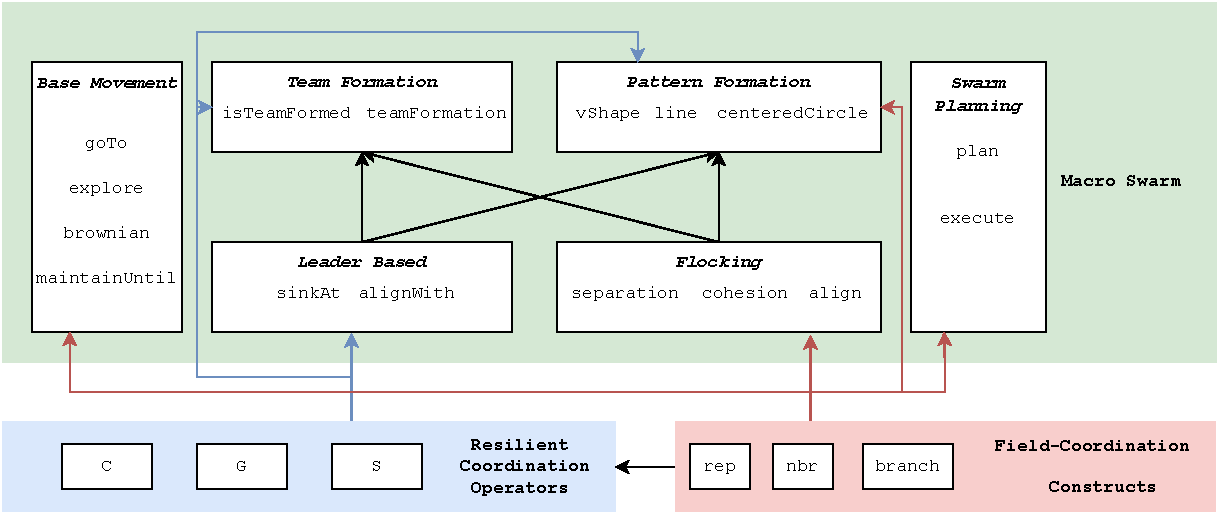
\includegraphics[width=\textwidth]{papers/coordination2023-macro/images/architecture.drawio.pdf}
  \caption[\MacroSwarm{}: architecture overview.]{\MacroSwarm{}: architecture overview. 
  The black boxes contained in the green rectangle 
  represent the main modules of the library.
  }\label{fig:architecture}
\end{figure}

This section presents the \MacroSwarm{} approach and \ac{api}.
%
In particular, we describe its overall architecture, and the main blocks exposed by the \ac{api}
 (summarized in \Cref{fig:architecture}), 
 which support the specification of a wide range of high-level swarm behaviours. 
%
The key idea in the design of \MacroSwarm{}  
 lies in the representation of a swarm behavioural unit 
 as a function mapping sensing and parameter fields 
 to actuation fields (often, velocity vectors).
%
We have organized the \ac{api}
 into multiple \emph{modules},
 capturing logically related sets of behaviours,
 and
 comprising more fundamental and reusable sets of behaviours
 as well as more application-specific sets (e.g., related to movement or team formation).
%This design process has resulted in an \ac{api} divided into several layers,  
% where each layer has a clear concern related to collective behaviour in swarms described in the following paragraphs.
 
% In particular, \textbf{Movement Blocks} discusses the basic movements 
%  associated with a group of agents that don't require coordination between them in order to be performed.
% %
% \textbf{Flocking blocks}, on the other hand, 
%  introduces the first elements of coordination, 
%  namely the one used to create swarms of agents according to some boids model (e.g., Reynolds \cite{DBLP:conf/siggraph/Reynolds87}). 
% %
% Section \textbf{Leader Based blocks} presents a set of \acp{api} 
%  where a leader is used to coordinate a group of followers.
% % 
% Another important aspect discussed in \textbf{Pattern formation blocks} 
%  is the formation of spatial patterns, that are different from \textbf{Team formation blocks}
%  in which the agents are not required to move in a specific spatial configuration but only 
%  to be grouped together following a specific rule.
% %
% Finally, the last section \textbf{Swarm Planner blocks} 
%  shows how to sequentially combine high-level collective patterns according to a swarm plan.
%\meta{General idea: we have a set of blocks that can be composed to create swarm behaviours. Here we classify the blocks in terms of their functionality, and we show how they can be composed to create complex behaviours. We present the blocks in several subsections}

\subsubsection{Movement blocks}\label{subsec:base}
%
These blocks control the movement of individual agents within the swarm. 
%These blocks are responsible for determining how agents move and interact with their environment. 
The simplest movement expressible 
 with \MacroSwarm{} is a collective constant movement (\Cref{fig:constant}), 
 described through a tuple 
 %(\lstinline|Point2D(x, y)|) or a
 %triple (
 like \lstinline|Vector(x,y,z)|
 that devises the velocity vector of the swarm:
\begin{lstlisting}
Vector(2.5, 0, 0) // a constant field which is the same for all the agents
\end{lstlisting}
This vector must then be appropriately mapped 
 the right electrical stimulus for the underlying engine platform
 of the mobile robot of interest.
On top of that, 
 this module exposes several blocks to explore an environment. 
%
Particularly, the \lstinline|brownian| block produces a random velocity vector 
 for each evaluation of the program. 
%
In addition to that simple logic, 
 there are movements based on GPS like \lstinline|goTo| 
 (produces a velocity vector that eventually moves the system to sink at one single point)
 and \lstinline|explore| 
 (produces a velocity vector that let the system explore a rectangle defined through \lstinline|minBound| and \lstinline|maxBound|).
%
The last one is based on temporal blocks, 
  like \lstinline|maintainTrajectory| and \lstinline|maintainUntil|.
%
The former allows the systems to maintain a certain velocity for the time specified. 
 At that moment, a new velocity is generated according to the given strategy. 
% 
The latter, instead, is used to maintain a certain velocity until a condition is met 
 (e.g., a target position is reached).
%
This module also exposes an \lstinline|obstacleAvoidance| block (\Cref{fig:obstacle-avoidance}), which creates a vector pointing away from obstacles.

Even if these blocks are quite simple, 
 it is still possible to combine them to create interesting behaviours. 
For instance, program 
\begin{lstlisting}
(maintainVelocity(browian()) + obstacleAvoidance(sense("obs"))).normalize
\end{lstlisting}
expresses a collective behaviour in which the nodes will explore the environment,
 while avoiding any obstacles perceived through a sensor. 
Notice how the composition is achieved by simply summing the computational fields produced by the sub-blocks.
%
Expression \lstinline|v.normalize| yields \lstinline|v| as a unit vector (of length 1), while keeping the same direction---useful when combining several vectors together.
% since we want to keep the direction of the vector but we want to reduce its magnitude.
%% @metaphori and @mviroli it makes sense to have a table with the blocks and a short description of them?
%
A summary of the blocks exposed by this module is reported in the following listing:
\begin{lstlisting}
// Movement library
def brownian(scale: Double): Vector
// GPS Based
def goTo(target: Point3D): Vector
def explore(minBound: Point3D, maxBound: Point3D): Vector
// Temporal Based
def maintainTrajectory(trajectory: => Vector)(time: FiniteDuration):Vector
def maintainUntil(direction: Vector)(condition: Boolean): Vector
// Obstacle Avoidance
def obstacleAvoidance(obstacles: List[Vector]): Vector
\end{lstlisting}

\subsubsection{Flocking blocks}\label{subsec:flockig} 
In a swarm-like system, 
 it is often necessary to coordinate the movement of the entire swarm, 
 rather than just individual agents, to achieve emergent behaviours,
 and ensure that the nodes move cohesively, avoid collisions, 
 and strive to be aligned in a common direction. 
% 
Therefore, in this module, 
 we have implemented the main blocks to support the \emph{flocking} of agents. 
% 
Several models are available in the literature for this purpose.
 Particularly, \MacroSwarm{} exposes 
 the Vicsek~\cite{VicsekModeling1995}, 
 Cucker-Smale~\cite{CuckerSmaleModeling2007}, 
 and Reynolds (\Cref{fig:flock})~\cite{DBLP:conf/siggraph/Reynolds87} models. 
% 
%We chose the first one because it is simple 
% and only require knowledge of the neighbours' velocity. 
% 
%The second one is an extension of the Vicsek model and 
% requires knowledge of the neighbours' relative distance as the Reynolds rules.
% more discussion here
We have also exposed the individual blocks to implement Reynolds, 
 which are \lstinline|cohesion|, \lstinline|separation|, and \lstinline|alignment|. 
% 
These blocks can be used individually by higher-level blocks to implement specific behaviours 
 (e.g., following a leader while avoiding collisions). 

Another essential aspect that emerges at this level is the concept of a \emph{variable neighbourhood}. 
%
Indeed, it may happen that the logical neighbourhood model used by aggregate computing 
 does not match the one used to coordinate the agents. 
 Thus, the node's visibility can be more \emph{restrictive} or \emph{extensive} 
 according to the neighbourhood model applied. 
%
In particular, in the case of Reynolds, 
 it is typical for the separation range to be different from that of alignment. 
% 
Therefore, the flocking blocks accept a ``query'' strategy towards a variable neighbourhood.
 The main implementation of these queries are:
\begin{itemize}
  \item \lstinline|OneHopNeighborhood|: the same as the aggregate computing model;
  \item \lstinline|OneHopNeighborhoodWithinRange(radius: Double)|: it takes all the nodes in the neighbourhood within the given range.
  %\item \lstinline|LongRangeNeighborhood(radius: Double)|: it expands the range of 
  %  aggregate computing communication by spawning 
  %  an aggregate process for each node that expands itself within the range passed.
\end{itemize}

The flocking models are typically described 
 by an iterated function in which the velocity at time $t+1$ depends on the velocity at time $t$.
Taking as an example the Vicsek rule, it is described as:
$ v_i(t + 1) = \frac{\sum_{j \in \mathcal{N}}v_j(t) }{|\mathcal{N}|} + \eta_i(t)$
where $\mathcal{N}$ is the neighbourhood of the node $i$ at time $t$, 
 $v_i(t)$ is the velocity of the node $i$ at time $t$, 
 and $\eta_i(t)$ is a random vector that models the noise of the model.
%
For this reason, 
 each block receives the previous velocity field as a parameter, 
 rather than encoding it internally within each block. 
% 
This is because the previous velocities 
 may be influenced by other factors, 
 such as constant movements or a target position. 
%
%To express changes in the computational field 
% in the aggregate computing context, the \lstinline|rep| operator 
% can be used (refer to \Cref{sec:background} for more details). 
Typical usage of this operator follows the following schema:
\begin{lstlisting}
rep(initialVelocity) { oldVelocity => flockingOperator(oldVelocity, ..) }  
\end{lstlisting}
For example, 
 the following program describes a collective movement 
 in which the nodes try to reach the position \texttt{(x,y)} while maintaining a distance of \texttt{k} meters from one another:
\begin{lstlisting}
rep(Point2D.Zero) {
  v => (goTo(Point2D(x, y)) + 
       separation(v, OneHopNeighbourhoodWithinRange(k))).normalize
}
\end{lstlisting}
%Until this level, 
% the self-organizing blocks of aggregate computing 
% are used only within the extended neighbourhood (through the aggregated processes).

\subsubsection{Leader-based blocks}\label{subsec:leader}
These blocks allow agents to follow a designated leader.
The idea behind leadership in swarm systems is that a leader 
 can act as a coordinator, influencing the followers that recognize it as such. 
% 
In the context of aggregate computing, 
 leaders are typically defined as Boolean fields holding \lstinline|true| for leaders 
 and \lstinline|false| for non-leaders. 
%
Leaders can be predetermined (i.e., nodes with certain characteristics), 
 virtual (i.e., nodes that do not actually exist in the system but are simulated for collective movement steering),
 or chosen in space (e.g., using the \lstinline|S| block---see \Cref{sec:background}). %, which seeks to create spatial partitions of the system). 
% 
A leader can be thought of as creating an \emph{area of influence}, affecting the actions of its followers.
%This leader creates a field of influence in which actions chosen by it can be taken.


Currently, we have identified \lstinline|alignWithLeader| and \lstinline|sinkAt| (\Cref{fig:towards-leader}) 
 as essential blocks. 
%
The former propagates the leader's velocity throughout 
 its area of influence (e.g., via \lstinline|G|---see \Cref{sec:background}),
 with followers adjusting their velocity to it. 
%
However, sometimes it may also be desirable 
 to create a sort of attraction towards the leader, 
 so that the nodes remain cohesive with it. 
For this reason, the  \lstinline|sinkAt| block creates a computational field 
 in which nodes tend to move towards the leader. 
% 
These blocks are useful for higher-level blocks, 
 such as those associated with the creation of teams or spatial formations.
 
\subsubsection{Team formation blocks}\label{subsec:team}
These blocks allow agents to form \emph{teams} or sub-groups within the swarm,
 useful e.g. for work division
 or situations requiring intervention by few agents.
% 
%Team formation is essential in cases where work division  is necessary or when specific situations arise. 
% 
In general, the formation of a team creates a ``split'' in the swarm logic, 
 conceptually creating multiple swarms with potentially different goals (cf. \Cref{fig:team}).
 %
One way to create teams is by using the \lstinline|branch| construct (see \Cref{sec:background}). 
%This allows for the creation of two non-communicating spatial zones. 
For example, the following program,
\begin{lstlisting}
def alignVelocity(id: Int) = 
  alighWithLeader(id == mid(), rep(browian())(x => x)
branch(mid() < 50) { alignVelocity(0) } { alignVelocity(50) }
\end{lstlisting}
creates two groups, each of which follows a certain velocity dictated by the leaders (0 and 50).

Other times, one needs to create teams based on the spatial structure of the network or when certain conditions are met. 
%
The \lstinline|teamFormation| block supports this scenario. %% todo ad reference to the last listing 
By internally using \lstinline|S|, it allows for the creation of teams based on certain spatial constraints expressed through parameters \lstinline|intraDistance| (i.e., the distance between team members) and
 \lstinline|targetExtraDistance| (i.e., the size of the leader's area of influence). 
%
It is also possible to create teams based on predetermined leaders, denoted explicitly by Boolean fields. %(instead of leveraging \lstinline|S| under the hood).
%
Moreover, since team formation may take time to complete, or require conditions to be met (e.g., that at least $N$ members are present, or that the minimum distance between all nodes is less than a certain threshold),
 we also parameterise \lstinline|teamFormation| by a \lstinline|condition| predicate. 
 %or that the number of nodes near the leader is greater than 10, %etc. 
%
An example of built-in predicate is \lstinline|isTeamFormed|, which verifies that each node under 
 the influence of the leader has a \lstinline|necessary| a number of neighbours
 within a \lstinline|targetDistance| radius.
%
%This can be combined with \lstinline|teamFormation| in the following way:
An example is as follows.
\begin{lstlisting}
teamFormation(targetIntraDistance = 30, // separation
  targetExtraDistance = 300, // influence of the leader
  condition = leader => isTeamFormed(leader, targetDistance = 40)
).velocity // use the velocity vector to create the Team
\end{lstlisting}
Each team must refer to a single leader, 
 who can coordinate the associated nodes 
 (using the APIs exposed by the \textbf{Leader Based Block}). 
In particular, to execute a certain behaviour within a team, 
 the \lstinline|insideTeam| method must be used. 
 Given the ID of the leader to which a node belongs, 
 this method can define the movement logic relative to that leader.
%
For instance, this code aligns the followers with a velocity generated by a leader, 
\begin{lstlisting}[xrightmargin=-3.4pt]
team.insideTeam{leader => alignWithLeader(leader)(rep(brownian())(x => x))}
\end{lstlisting}
%In the following, there is the complete API for this layer:
%\begin{lstlisting}
%// Team formation API
%def teamFormation(
%  intraDistance: Double, extraDistance: Double, 
%  condition: Boolean => Boolean // leader field from the condition field
%): Team
%def isTeamFormed(source: Boolean, targetDistance: Double, necessary: Int): Boolean
%// Team abstraction
%class Team(leader: ID, formed: Boolean, nodeVelocity: Point3D) {
%  def insideTeam(velocityGenerator: ID => Point3D): Point3D
%}
%\end{lstlisting}

\begin{figure}[t]
\centering
\begin{subfigure}{0.32\textwidth}
  \centering
  {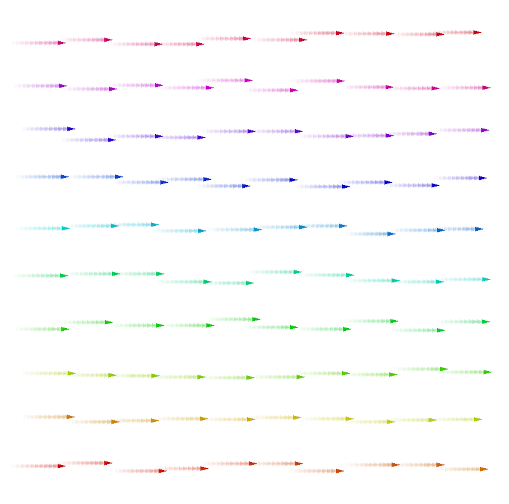
\includegraphics[width=\textwidth]{papers/coordination2023-macro/images/constant.png}}
  \caption{}
  \label{fig:constant}
\end{subfigure}
\hfill
\begin{subfigure}{0.32\textwidth}
  \centering
  {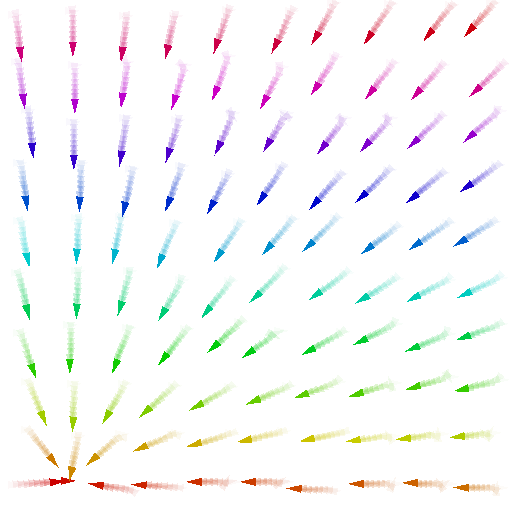
\includegraphics[width=\textwidth]{papers/coordination2023-macro/images/towards-leader.png}}
  \caption{}
  \label{fig:towards-leader}
\end{subfigure}
\hfill
\begin{subfigure}{0.32\textwidth}
  \centering
  {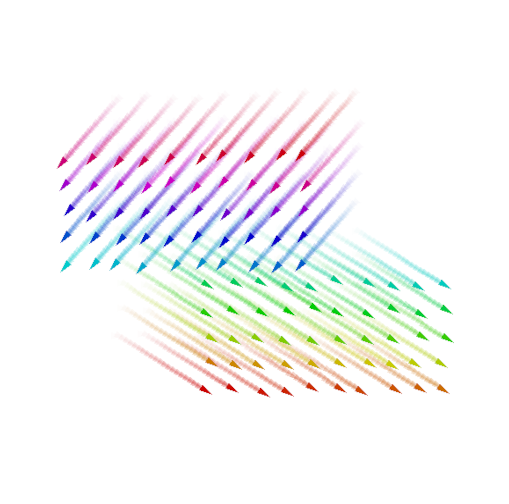
\includegraphics[width=\textwidth]{papers/coordination2023-macro/images/branching.png}}
  \caption{}
  \label{fig:team}
\end{subfigure}
\hfill
\begin{subfigure}{0.32\textwidth}
  \centering
  {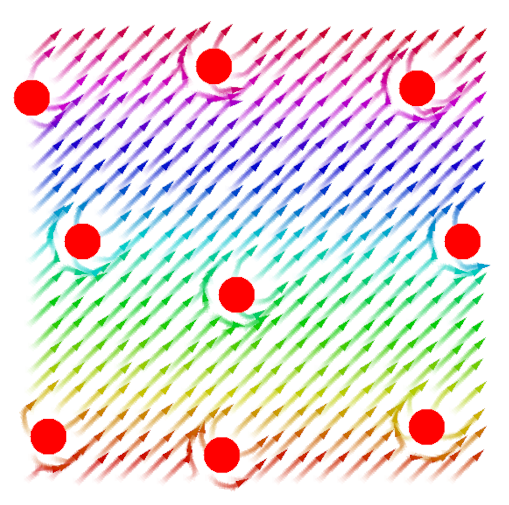
\includegraphics[width=\textwidth]{papers/coordination2023-macro/images/obstacle-avoidance.png}}
  \caption{}
  \label{fig:obstacle-avoidance}
\end{subfigure}
~
\begin{subfigure}{0.32\textwidth}
  \centering
  {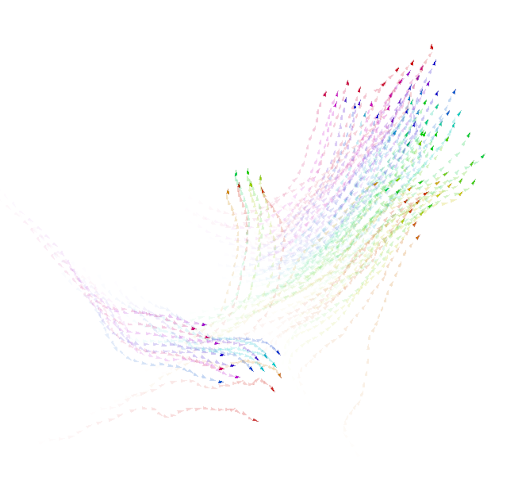
\includegraphics[width=\textwidth]{papers/coordination2023-macro/images/flock.png}}
  \caption{}
  \label{fig:flock}
\end{subfigure}
\caption{Overview of swarm behaviours expressible with \MacroSwarm{}.}\label{fig:movement-overview}
\end{figure}

\subsubsection{Pattern formation blocks}\label{subsec:pattern}
%they enable agents to create complex spatial patterns. 
Team formation blocks can be used to create groups of agents with certain characteristics.
%
However, sometimes we are also interested in the \emph{spatial structure} of the group. 
%
In swarm behaviours, the spatial structures of the teams can be instrumental for performing certain tasks (e.g., coverage or transportation tasks).
% 
In \MacroSwarm{} some of the most idiomatic spatial structures are available. 
% have been implemented to show how they can be easily integrated into this framework. 
%

The implementation is as follows. First, the formation of structures is based on the presence of a leader that
 %it is not a must since there are other approaches in which this is done in a distributed way,
 %but for simplicity, we chose to use a leader to perform this coordination task.  
collects the hop-by-hop distances 
 of their followers (leveraging \lstinline|G| and \lstinline|C|) and
 sends them a direction in which they should go to form the required structure (using \lstinline|G|).

The structures currently supported (\Cref{fig:formations}) are v-like shapes (\lstinline|vShape|), lines (\lstinline|line|), and circular formations (\lstinline|centeredCircle|). 
 These structures are \emph{self-healing}: if there is a disturbance 
 of the structure, 
 the group tends to reconstruct itself and return to a stable structure. 
Additionally, it is assumed that the leader has his own speed logic. 
 In this way,
 the group will follow the leader maintaining the chosen structure. 
%\meta{Here we can put a figure that summarizes the relation between the blocks and also with the standard AC blocks.}
\begin{figure}[t]
  \centering
  
\includegraphics[width=0.9\textwidth]{papers/coordination2023-macro/images/shapes.png}
  \caption{Examples of the supported patterns. From left to right: 
   line formation, v-like formation, and
   circular formation.
  }
   \label{fig:formations}
\end{figure}
  
\subsubsection{Swarm Planning blocks}\label{subsec:planner} %% I dunno if we wanna discuss this

With the previous blocks available, there is a need for a handy mechanism to express a series of \emph{plans} that 
 change over time and move the swarm towards different targets. 
%
For this reason, \MacroSwarm{} also exposes the concept of \emph{swarm planning}. 
The idea is to express a series of plans (or missions)
 defined by a \emph{behaviour} 
 (i.e., the logic of production of a velocity vector) 
 and a \emph{goal} (defined as a boolean predicate condition). 
%
At any given time, the swarm will be executing a certain sub-plan, 
 which will be considered complete only when the boolean condition is satisfied. 
%
At this point, the swarm will follow the next objective described by the overall plan.
%
The exposed API allows for the creation of these collective plans in the following way:
\begin{lstlisting}
execute.once {
  plan(goTo(goalOne).endWhen(isClose(goalOne)),
  plan(goTo(goalTwo).endWhen(isClose(goalTwo)),
}.run() // will trigger the execution of the plan
\end{lstlisting}
This snippet creates a plan 
 in which the nodes will first go to \lstinline|goalOne|, 
 and once reached (\lstinline|isClose| verifies that the node is close enough to the point passed), 
 it will move on to the next objective \lstinline|goalTwo|.
Since it is specified that the mission is executed \lstinline|once|, 
 after the completion of the last plan, the group will stop moving.
To make the group repeat the plan, 
 the \lstinline|repeat| method can be used instead of \lstinline|once|.
%
Note that there is no coordination between agents in the above code, 
 but you can enforce it using lower-level blocks (e.g., flocking or team-based behaviours).
%
For example, \MacroSwarm{} enables describing a swarm behaviour where:
(i) a group of nodes gathers around a leader,
(ii) the leader brings the entire group towards the \lstinline|goalOne|,
(iii) the leader brings the entire group towards the \lstinline|goalTwo|.
%
This can be described using the following code:
\begin{lstlisting}[xrightmargin=-5pt]
execute.once( // if it is repeated, you can use `repeat'
  plan{sinkAt(leaderX)}.endWhen{isTeamFormed(leaderX, targetDistance=100)},
  plan(goTo(goalOne)).endWhen{ G(leaderX, isClose(goalOne), x => x)},
  plan(goTo(goalTwo)).endWhen{ G(leaderX, isClose(goalTwo), x => x)},
).run()
\end{lstlisting}
The use of \lstinline|G| in this way is a recurrent pattern, 
 and in \scafi{} it is exposed through the \lstinline|broadcast[T](center: Boolean, value: T): T| block.
 
\section{Evaluation}
\label{sec:eval}

To validate the proposed approach and \ac{api} we define a simulated \emph{find-and-rescue} case study,
to show 
the ability of \MacroSwarm{} to express complex swarm behaviours (\Cref{subsec:case-study}). 
Then, we discuss the results of the case study and the applicability of the proposed approach in real-world scenarios (\Cref{subsec:discussion}).

\subsection{Case Study: Find and Rescue}\label{subsec:case-study}
In our scenario, we want a fleet of drones to patrol a spatial area.
% 
In the area, dangerous situations may arise (e.g., a fire breaks out, a person gets injured, etc.). 
%
 In response to these, a drone designated as a \emph{healer} 
 must approach and resolve them. %how this should be resolved is beyond the scope of this case study). 
%
Exploration must be carried out in groups composed of \emph{at least} one 
 healer and several \emph{explorers}, who will help the healer identify alarm situations.

\subsubsection{Goal}
The goal of the proposed case study is to demonstrate the effectiveness of the proposed \ac{api} in terms of expressiveness (i.e., the ability to describe complex behaviours easily) and correctness (i.e., the described behaviour collectively does what is expressed). 
%
For the first point, since it is a qualitative metric, we will show the development process that led to the implementation of the produced code, demonstrating its ease of understanding. 
%
For the second point, since deploying a swarm of drones is costly, we will make use of simulations to verify that the program is functioning correctly both qualitatively (e.g., observing the graphical simulation) and quantitatively (i.e., extracting the necessary data and computing metrics that allow us to understand if the system behaves as it should).
%
%The area to be monitored is a square 1000x1000 meters in size. 
%

\subsubsection{Setup}
Initially, 50 explorers and 5 healers are randomly positioned in an area of $1 km^2$. 
 Each drone has a maximum speed of approximately 20 km/h and a communication range of 100 meters.
%
The alarm situations are randomly generated at different times %every minute 
 within the spatial area in a $[0,50]$ minutes time-frame. 
%
% After 50 minutes, no more alarm situations will be generated. 
%
Each simulation run lasts 90 minutes, 
 during which we expect the number of alarm situations to reach a minimum value.
The node should form teams of at least one healer and several explorers, maintaining a distance of at least 50 meters between the node and the leader

\subsubsection{Implementation details}
\begin{figure}[t]
\begin{subfigure}{0.29\textwidth}
  \centering
  \fbox{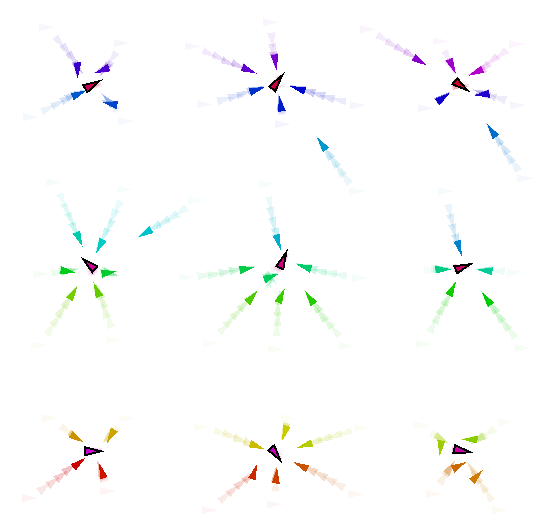
\includegraphics[width=\textwidth]{papers/coordination2023-macro/images/team-formation.png}}
  \caption{Team formation}
  \label{fig:team-formation}
\end{subfigure}
\hfill
\begin{subfigure}{0.29\textwidth}
  \centering
  \fbox{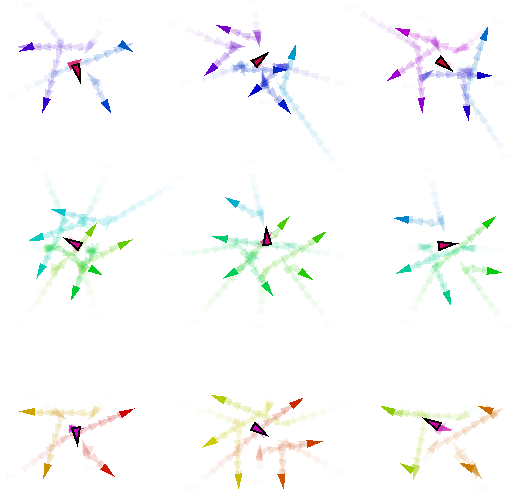
\includegraphics[width=\textwidth]{papers/coordination2023-macro/images/circle-formation.png}}
  \caption{Circle formation}
  \label{fig:circle-formation}
\end{subfigure}
\hfill
\begin{subfigure}{0.29\textwidth}
  \centering
  \fbox{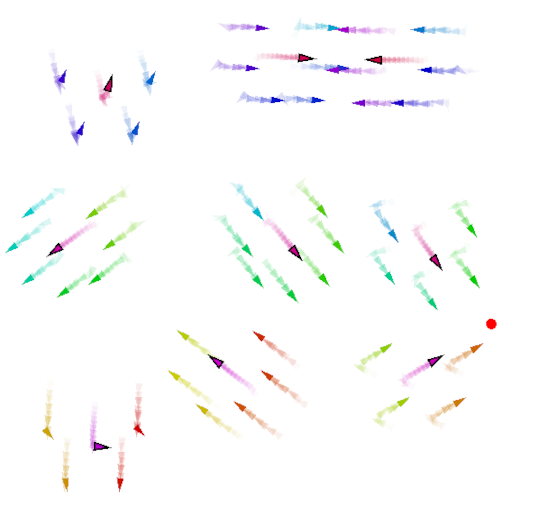
\includegraphics[width=\textwidth]{papers/coordination2023-macro/images/explore.png}}
  \caption{Explore}
  \label{fig:explore}
\end{subfigure}
\caption[\MacroSwarm{} graphical simulations example]{The first phases of the scenario described in \Cref{sec:eval}. 
 At the beginning, the system is split into teams; 
 afterwards, the teams assume a spatial formation (circular, in this case);
 finally, the teams start exploring the overall area.}\label{fig:scenario}
\end{figure}

To structure the desired swarm behaviour, 
 we break the problem into parts:
\begin{enumerate}
  \item the swarm must split into teams regulated by a healer, who works as a \emph{leader} %in which at least one leader is present 
   (\Cref{fig:team-formation});
  \item teams must assume a spatial formation promoting the efficiency of the exploration (\Cref{fig:circle-formation});
  \item the teams must explore the overall area (\Cref{fig:explore});
  \item when any node detects an alarm zone, it must point that to the healer;
  \item the healer node approaches the dangerous situation to fix it;
  \item then, the team should return to the exploration phase.
\end{enumerate}
%
We now describe the implementation of each part, leveraging the \MacroSwarm{} API. % and \scafi{} for the aggregate programming basic blocks.
First, for creating teams, we can use the \textbf{Team Formation} blocks:
\begin{lstlisting}
val teamFormedLogic = 
  (leader: ID) => isTeamFormed(leader, minimumDistance + confidence)
def createTeam() = 
  teamFormation(sense("healer"), minimumDistance, teamFormedLogic)
\end{lstlisting}
where \lstinline|minimumDistance| is the minimum distance between nodes during the 
 team formation phases and \lstinline|confidence| is the confidence interval 
 used to check if the team is formed through the \lstinline|isTeamFormed| method.
%
Each team then should follow the aforementioned steps, 
 expressible using the \textbf{Swarm Planning} \ac{api}: 
%
%Particularly, this set of instructions will produce the effects described in the above enumeration:
\begin{lstlisting}[xrightmargin=-2pt]
def insideTeamPlanning(team: Team): Vector = 
 team.insideTeam {
  healerId =>
   val leading = healerId == mid() // team leader
   execute.repeat(
    plan(formation(leading)).endWhen(circleIsFormed), // shape formation
    plan(wanderInFormation(leading)).endWhen(dangerFound), // exploration
    plan(goToHealInFormation(leading, inDanger)).endWhen(dangerReached), 
    plan(heal(healerId, inDanger)).endWhen(healed(dangerFound)) // healing
   ).run() // repeat the plan
 }
\end{lstlisting}
%Focusing on each of the steps, 
The first step is the formation of the teams, 
 based on method \lstinline|formation| which
 internally uses \lstinline|centeredCircle| 
  to place the nodes in a circle around the leader node. 
 Function \lstinline|circleIsFormed| verifies whether the nodes are in a circle formation, i.e., that the distance between any node and the leader is less than \lstinline|radius| (set to 50 meters in this scenario).
%
The second step is the exploration phase, 
 implemented by method \lstinline|wanderInFormation|, 
 which uses the \lstinline|explore| function to move the nodes to a random direction
 within given bounds while keeping the circle formation.
 This leverages \lstinline|centeredCircle|,  passing 
 the movement logic of the healer (leader) to the block.
Exploration will go on until someone finds a danger node, 
 denoted by predicate \lstinline|dangerFound|.
This internally uses \lstinline|C| and \lstinline|G| to collect the danger nodes' positions
 and share them within the team:
\begin{lstlisting}
def dangerFound(healer: Boolean): Boolean = {
  val dangerNodes = 
    C(sense("healer"), combinePosition, List(sense("danger")), List.empty)
  broadcast(healer, dangerNodes.nonEmpty)
}
\end{lstlisting}
%
The third step is the movement towards the danger node, 
 which is implemented by the \lstinline|goToHealInFormation| method, 
 which uses again the \lstinline|centeredCircle| function
 with a delta vector that moves the leader node towards the danger node.
\lstinline|inDanger| is computed similarly to \lstinline|dangerFound|, 
 but, in this case, the position will be shared instead. % of the presence of the danger node.
 \lstinline|dangerReached| is a Boolean field indicating if the healer node is close enough to the danger node.
The last step is the healing of the danger node, which is modelled as an actuation of the healer. % on the node in danger. 
 The rescue ends when the danger node is healed.
As a final note, we also want the nodes to be able to avoid 
 each other when they are too close, even if they are not in the same team.
 For this, we leverage the \textbf{Flocking} \ac{api} the \texttt{separation} block outside the team logic.
Then, the main program is as follows:
\begin{lstlisting}
val team = createTeam()
rep(Vector.Zero) { v =>
  insideTeamPlanning(team) + 
  separation(v, OneHopNeighbourhoodWithinRange(avoidDistance))
}.normalize
\end{lstlisting}
%The result is intuitive and therefore allows us to conclude that the created 
This program shows that the \ac{api} 
 is flexible enough to create complex behaviours handling various coordination aspects.
%

\subsubsection{Results}
We validated the results by effectively running simulations, 
 publicly available at \url{https://zenodo.org/badge/latestdoi/611692727}. 
 For this task, we used Alchemist~\cite{DBLP:journals/jos/PianiniMV13}, a general simulator for multi-agent and pervasive systems. % developed to support scenarios in pervasive computing, 
% but which is well suited to swarm behaviour contexts as well (the plots shown in \Cref{fig:scenario} were produced using this simulator).
%
We launched 64 simulation runs with different random seeds: 
 \Cref{fig:results} shows the average results obtained. 
We extracted the following data:
\begin{itemize}
  \item \emph{intra-team distance}:
   after an initial adjustment phase, 
   the system should converge to an average distance of 50 meters (\Cref{fig:distance});
  \item \emph{minimum distance between each node}: 
    as we want to avoid collisions, 
    the minimum distance between 
    two nodes should always be greater than zero (\Cref{fig:min_distance});
  \item \emph{number of nodes in danger}: 
   we expect the nodes in danger to increase 
   up to 50 minutes and then decrease, tending towards zero (\Cref{fig:danger}).
\end{itemize}
The results (\Cref{fig:results}) show that the system can achieve the expected outcomes.
\begin{figure}[t]
\centering
\begin{subfigure}{0.4\textwidth}
  \centering
  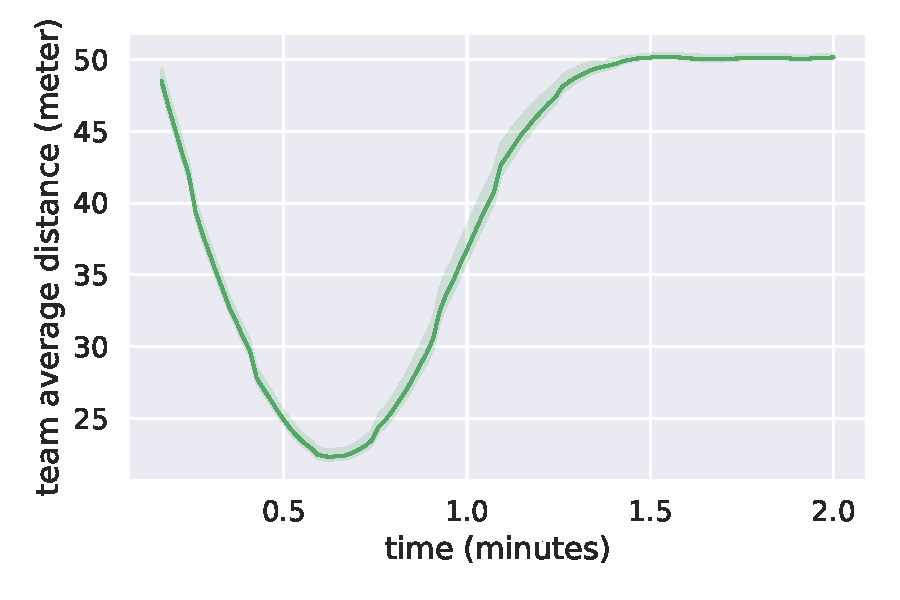
\includegraphics[width=\textwidth]{papers/coordination2023-macro/images/average_intra_team_distance}
  \caption{}
  \label{fig:distance}
\end{subfigure}
\hfill
\begin{subfigure}{0.4\textwidth}
  \centering
  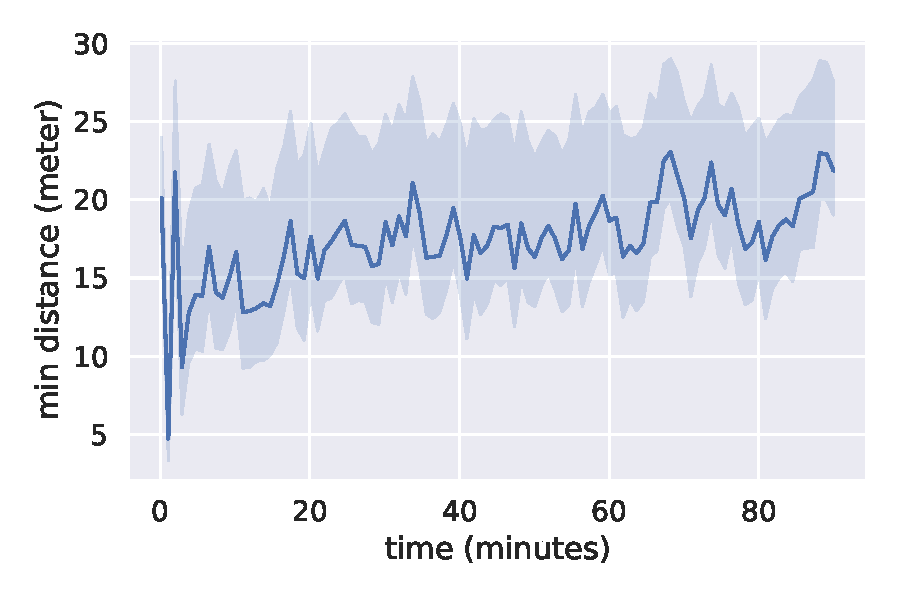
\includegraphics[width=\textwidth]{papers/coordination2023-macro/images/min_distance}
  \caption{}
  \label{fig:min_distance}
\end{subfigure}
\hfill
\begin{subfigure}{0.4\textwidth}
  \centering
  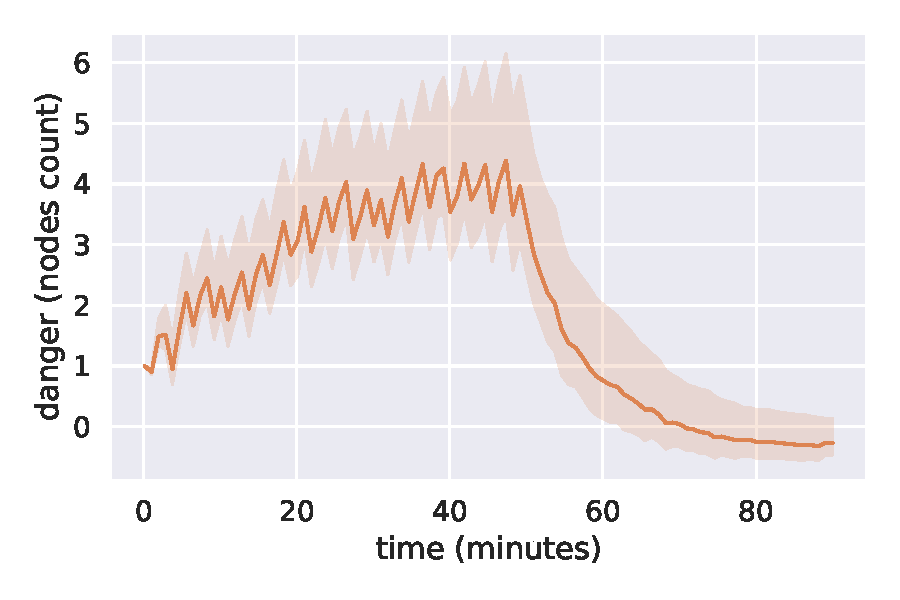
\includegraphics[width=\textwidth]{papers/coordination2023-macro/images/in_danger}
  \caption{}
  \label{fig:danger}
\end{subfigure}
\caption[Quantitative plots of the simulated scenario in \MacroSwarm{}.]{
  Quantitative plots of the simulated scenario. 
  \Cref{fig:distance} shows the average team distance in the first two minutes. 
  \Cref{fig:min_distance} shows the minimum distance between nodes. 
  \Cref{fig:danger} shows the nodes in danger through time. 
  Since we run several simulations, 
   the lines show the average values, whereas 
   the area around the lines shows the confidence interval throughout the simulations.
}\label{fig:results}
\end{figure}
%\meta{We will show the results of the simulations of the swarm behaviours, and the composition of the behaviours. }
%% figure composed of two subfigures

\subsection{Discussion}\label{subsec:discussion}
%
Despite its simplicity, 
this use case allowed us to demonstrate the capability of \MacroSwarm{}, both in qualitative terms (i.e., the produced code is simple and understandable) and quantitative terms (i.e., the data show that the swarm follows the given instructions correctly).

That being said, there are several things to consider when using the library in real-world contexts. Ours is a top-down approach, in which we have defined an evaluation and implementation system that is general enough to be executed in various multi-robot systems. Specifically, we require that at least: 
\emph{i)} nodes can perceive and interact with neighbours and approximate a direction vector to each of them; 
\emph{ii)} they can move in a specific direction with a certain velocity; and 
\emph{iii)} they can perceive distance and direction for certain obstacles.
%
As for point \emph{i)}, this can be developed using specific local sensors (e.g., range and bearing systems~\cite{DBLP:conf/antsw/BilalogluSAST22}), by using GPS, by approximating distances using cameras mounted on each drone, or by using Bluetooth direction finding~\cite{DBLP:conf/wcnc/SambuW22}.
% 
Concerning the point \emph{ii)} the velocity vector can be mapped to the motors of the UAVs, or the motor's wheels of the ground robots~\cite{DBLP:conf/icra/KorenB91}, so it can be easily implemented in real case scenarios.
%
Finally, concerning \emph{iii)}, there are several solutions for perceiving the direction of obstacles by leveraging various sensors, like \emph{\ac{lidar}} systems~\cite{DBLP:conf/icinfa/PengQZXLG15}.

That being said, we know that the reality gap for real-world scenarios could introduce divergences from the behaviours shown, as the used simulator, although general, does not simulate many aspects of reality, such as communication delay, friction, and possible perception errors. 
%
We aim to test the \ac{api} in more realistic simulators (like Gazebo~\cite{DBLP:conf/iros/KoenigH04}) or real systems as a future work.

\section{Related Work}
\label{sec:rw}

Related programming approaches for swarms 
 include 
 Meld~\cite{Meld2007},
 Buzz~\cite{DBLP:conf/iros/PinciroliB16},
 Voltron~\cite{Mottola2014voltron},
 TeCoLa~\cite{Koutsoubelias2016tecola},
 Dolphin~\cite{lima2018dolphin},
 Maple-Swarm~\cite{DBLP:conf/isola/KosakHBWHR20}, 
 PARoS~\cite{paros},
 Resh~\cite{DBLP:conf/icra/CarrollNS21}, 
 and \cite{DBLP:conf/iros/YiDLD0WY20}.
% MORE? Karma, COMETS? WOSP 
%
%These are reviewed in the following,
% where we distinguish two main groups: those based on decentralised execution,
% and those based on centralised task orchestration.
%
In the following, we review the works that are more related to \MacroSwarm{},
 which are those for expressing \emph{decentralized} behaviours.
 
%\subsubsection*{Decentralised approaches.}

Buzz~\cite{DBLP:conf/iros/PinciroliB16}
 is a mixed imperative-functional language for programming swarms.
%
%It provides primitives for both individual robots and whole swarms.
%
%Indeed, in Buzz, 
In Buzz, swarms are first-class abstractions:
 they can be explicitly created,
 manipulated,
 joined (e.g., based on local conditions),
 and used as a way to address individual members (e.g., for tasking them). %e.g., to make them perform certain operations.
%
For individual robots, 
 the language provides access to local features
 and the local set of neighbours, for interaction.
%
For swarm-wide consensus, 
 a notion of \emph{virtual stigmergy} is leveraged,
 based on distributed tuple spaces.
%
Buzz is designed to be an extensible language, since new primitives can be added.
%
Indeed, Buzz is based on a set of quite effective but ad-hoc mechanisms.
%
By contrast, \MacroSwarm{} uses few general and expressive primitives, 
  and supports swarm programming
  through a library of reusable, composable blocks.
%
%The compositionality advocated in Buzz is 
% mostly in terms of modularity (i.e., the possibility to define and reuse functions defined within modules); by contrast, \MacroSwarm{} leverages the functional compositionality of fields to combine whole behaviours.
%
Additionally, \MacroSwarm{} can leverage theoretical results from field calculi~\cite{DBLP:journals/jlap/ViroliBDACP19,DBLP:journals/tomacs/ViroliABDP18}, making programs amenable for formal analysis.


Voltron~\cite{Mottola2014voltron} is a programming model for team-level design of drone systems. It represents a group of individual drones through a \emph{team abstraction}, which is responsible for the overall task. The details of individual drone actions and their timing are delegated to the platform system during runtime. The programmer issues \emph{action commands} to the drone team, along with \emph{spatio-temporal constraints}. The tasks in Voltron are associated with spatial locations, and the team self-organises to populate \emph{multisets of future values} that represent the task's eventual result at a specific location. 
%
However, Voltron is imperative in nature, limiting the compositionality of team-level behaviours.


Meld~\cite{Meld2007} is a logic-based language for programming modular ensembles,
for systems where communication is limited to immediate neighbours. 
%It was inspired by a similar language called P2, which is used for overlay networks. 
%Meld is a macroprogramming approach, i.e., it aims to simplify the coordination of robot ensembles by taking a global perspective to programming, where macroprograms are compiled into microprograms deployed to individual robots.
%
It leverages 
\emph{facts with side-effects} to handle actuation, 
\emph{production rules} to generate new facts from existing facts, 
and \emph{aggregate rules} to combine multiple facts into one fact by folding (e.g., maximization or summation).
%
The runtime deals with communication of facts and removal of invalidated facts.
%
The declarativity and logical foundation 
 make Meld an interesting macroprogramming system;
 however, it is not clear how it can scale with the complexity of general swarm behaviour.
%
Indeed, it is mainly adopted for shape formation and self-reconfiguring ensembles.

Finally, we mention another category of related works, which are \emph{task orchestration languages} for swarms (e.g.,  TeCoLa~\cite{Koutsoubelias2016tecola},
 Dolphin~\cite{lima2018dolphin},
 Maple-Swarm~\cite{DBLP:conf/isola/KosakHBWHR20}, 
 PARoS~\cite{paros},
 Resh~\cite{DBLP:conf/icra/CarrollNS21}, 
 and \cite{DBLP:conf/iros/YiDLD0WY20}): they adopt quite a different approach that leverages centralized entities to control the activity of the swarm members based on the provided task descriptions.
%

 
%\subsubsection*{Centralised orchestration approaches}
%
%In \MacroSwarm{}, 
% a program provides a description of the collective tasks,
% but also acts as a control program for the individual agents,
% and is hence executed in a decentralised fashion.
%%
%In the following, we review task orchestration languages for swarms, which adopt a quite different approach that leverages centralised entities to control the activity of the swarm members based on the provided task descriptions.
%
%TeCoLa~\cite{Koutsoubelias2016tecola} is a programming framework that is designed to coordinate robotic teams and is implemented in Python. 
%%
%It provides abstractions for controlling individual robots and teams of robots, with most of the team management activities being handled automatically in the background. 
%%
%The framework uses the concept of nodes, which possess resources and services consisting of methods and properties that can be remotely invoked using proxies. 
%%
%TeCoLa leverages the notion of a \emph{mission group}, i.e., a dynamic set of nodes that participate in a mission, controlled and monitored by a \emph{coordinator entity} like a leader node or command control center. A mission group can also be split into teams whose shape is managed automatically, based on a \emph{membership rule} that specifies the set of services that team members should support. 
%%
%When all team members provide a particular service, that service is said to be promoted at the \emph{team-level}, allowing it to be requested on the team itself, triggering a corresponding service request on all team members and returning a vector of results.
%
%PARoS~\cite{paros} is a Java framework for programming swarms that, similarly to the other reviewed approaches, provides an \emph{abstract swarm} abstraction, to support orchestration and spatial organisation of multiple robots. 
%%
%The \ac{api} provides various functions that include path planning, declaration of points of interest  (e.g., spatial locations that need to be inspected), enumeration swarm members, and event handling (e.g., to respond to robot failure).
%%
%The PARoS language combines elements from imperative, declarative, and event-driven programming.
%%
%At the execution level, PARoS uses a centralised coordinator, limiting the scalability of the approach.
%% see TABLE 1 from https://doi.org/10.1145/3197768.3197772
%
%Maple-Swarm~\cite{DBLP:conf/isola/KosakHBWHR20} (``Multi-Agent script Programming
%Language for multipotent Ensembles'')
%  is an approach to swarm programming
%  that is based on concepts like
%  agent groups (for addressing subsets of agents), 
%  virtual swarm capabilities, 
%  and hierarchical task plans.
%%
%Maple supports the orchestration of individual agents
% through tasks that are derived from a composition of context-oriented partial plans.
%%
%In Maple, compositionality is obtained by connecting partial plans, which are defined in terms of swarm capabilities--the analogue of collective behaviours in \MacroSwarm{}. 
%%
%%However, Maple does not provide a formal framework supporting  programming of swarm capabilities.
%%
%In \MacroSwarm{}, we directly support programming swarm capabilities by leveraging the field-based framework.
%
%Dolphin~\cite{lima2018dolphin} is a Groovy \ac{dsl} designed specifically for task-oriented programming for autonomous vehicle networks. 
%%
%In Dolphin, the main abstraction is the \emph{vehicle set}, which is a dynamic group of vehicles that can be manipulated using set operations and pick/release operators---similarly to swarms in Buzz.
%%
%In Dolphin, the macro-level program defines how groups of vehicles are formed and tasked, essentially supporting the orchestration of individual behaviours, which are specified separately.
%
%In~\cite{DBLP:conf/iros/YiDLD0WY20},
% a mixed decentralised-centralised actor-based framework
% is proposed for programming swarms.
%%
%The authors propose a \emph{collective actor} mechanism
% to centrally manage a swarm
% and provide primitives for high-level coordination
% (e.g., barrier synchronisation, branching and aggregation of swarms).
%%
%Though interesting, the approach -- unlike \MacroSwarm{} -- does not provide a well-defined programming model: instead, it is based on XML dialects to define actor configurations and task scripts.
%
%Resh~\cite{DBLP:conf/icra/CarrollNS21} is 
% a \ac{dsl} for orchestration of multi-robot systems.
%%
%It leverages 
% the notion of a \emph{task} as a compositional block,
% robot capabilities (which are to be advertised by the robots),
% and spatiotemporal primitives (e.g., for waiting for events, specifying the location where a task is to be executed, etc.).
%%
%However, Resh is not Turing-complete, to simplify synthesis of task orchestration programs.

\section{Conclusion and Future Work}
\label{sec:conc}

We presented \MacroSwarm{},
 a framework 
 for top-down swarm programming
 that provides composable blocks 
 capturing common decentralized swarm behaviours.
%
It builds on aggregate computing,
 a formally-grounded field-based coordination paradigm,
 and is implemented on top of the \scafi{} toolkit/\ac{dsl}.
%
We show through examples and a simulated case study
 that the approach is compositional, practical, and expressive.

As future work,
 we plan to make the \ac{api} more comprehensive,
 by covering all the main patterns from notable taxonomies of swarm behaviour~\cite{DBLP:journals/swarm/BrambillaFBD13}.
%
Additionally, it would be interesting to investigate approaches for synthesizing compositions of \MacroSwarm{} blocks, e.g., by following the reinforcement learning-based approach of~\cite{DBLP:conf/coordination/AguzziCV22}.
%
Last but not least, we would like to deploy and test the framework on real test beds.

\printbibliography
